
% subsection 4.6
\subsection{Stage 6: Results}
Esta sección presenta los resultados obtenidos mediante la ejecución del protocolo de búsqueda SMS.\@ Inicialmente, se proporciona una descripción general de los datos correspondientes a los Estudios Primarios Seleccionados (SPS's).
Esta descripción abarca aspectos como el origen de los estudios, el año de publicación, la estrategia de búsqueda, los índices de calidad, su relación con las preguntas de investigación (RQs) y los temas respectivos, y las palabras clave. Finalmente, se presenta una nube de palabras generada a partir de las palabras clave de las SPS.\@
Es importante recordar que la asociación entre los SPS y los temas se estableció mediante la clasificación detallada descrita en la sección~\ref{subsec:clasificacion-de-estudios}. Por consiguiente, las preguntas de investigación también se asociaron, ya que los temas siguen una estructura específica dentro de ellas.
Además, se identificó la asociación entre las principales palabras clave de SMS y los títulos de las secciones, resúmenes y palabras clave de todos los SPS.\@

% sub-subsection 4.6.1
\subsubsection{General Description of the SPSs (Selected Primary Studies)}
El proceso de búsqueda y filtrado de estudios dio como resultado la identificación de 181 SPS, como se muestra en la Tabla~\ref{table:selected_primary_studies}.

\begin{figure}[htbp]
	\centering
	\vspace{10pt}
	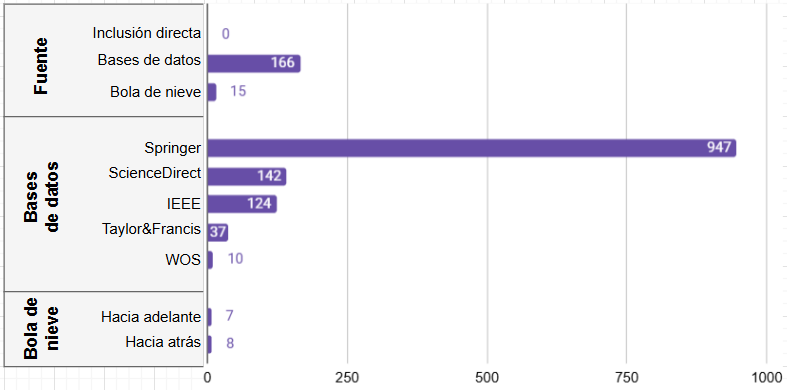
\includegraphics[scale=0.7]{resources/images/Planeacion/procedencia_datos.png}
	\vspace{6pt}
	\caption{SPSs by source and search strategy.}\label{fig:SPSsByProcedence}
\end{figure}

Estos SPS se obtuvieron de bases de datos digitales, identificadas en el SMS mediante diferentes estrategias. La figura~\ref{fig:SPSsByProcedence} muestra el número de estudios recuperados de diversas fuentes y los detalles de las estrategias de búsqueda en bases de datos y de bola de nieve. Independientemente de la fuente, el 91,7\% de los SPS se encontraron mediante la búsqueda en bases de datos, mientras que el 13,16\% restante se identificó mediante la estrategia de bola de nieve.
Independientemente de la estrategia de búsqueda en bases de datos, la figura \ref{fig:SPSsByProcedence} muestra que, de los 99 estudios identificados mediante la búsqueda en bases de datos, el 50,59\% se encontraron en la base de datos ACM, el 24,24\% en ScienceDirect y el 17,17\% en Springer. Entre los 15 SPS identificados mediante bola de nieve, el 40\% se descubrieron mediante bola de nieve hacia atrás y el 60\% mediante bola de nieve hacia adelante.

\begin{figure}[htbp]
	\centering
	\vspace{10pt}
	\includegraphics[scale=0.7]{resources/figures/Venn.png}
	\vspace{6pt}
	\caption{Relationship of SPSs with the research questions.}
	\label{fig:SPSsByRQs}
\end{figure}

Considering the relationships of the SPSs with the RQs, Figure \ref{fig:SPSsByRQs} shows that 100.00\% of the SPSs are related to RQ1, while 24.56\% of the SPSs are simultaneously related to both RQs. Consequently, the remaining 75.44\% are exclusively associated with RQ1. This indicates that no SPS is related solely to RQ2.

\begin{figure}[htbp]
	\centering
	\vspace{10pt}
	\includegraphics[scale=0.7]{resources/figures/SPSsByTopic.jpg}
	\vspace{6pt}
	\caption{Relationship of SPSs with research topics.}
	\label{fig:SPSsByTopics}
\end{figure}

Figure \ref{fig:SPSsByTopics} shows the topics defined during the planning stage for each research question and the number of SPSs inclusively associated with each topic. It is essential to note that one SPS may be linked to multiple topics simultaneously. In this sense, Figure \ref{fig:SPSsByTopics} displays the 12 topics associated with RQ1, where the topic ``Grid Computing'' is the most frequent at 34.21\%. In contrast, the least frequent topics are ``Java'' and ``Checkpointing,'' both at 0.87\%. On the other hand, Figure \ref{fig:SPSsByTopics} also shows the three topics associated with RQ2, where the topic ``Research'' is the most frequent at 16.67\%, while the least frequent is ``industry'' at 2.63\%.

\begin{figure}[htbp]
	\centering
	\vspace{10pt}
	\includegraphics[scale=0.7]{resources/figures/SPSsBYearsAndIndexes.jpg}
	\vspace{6pt}
	\caption{Relationship of SPSs with years of publication and quality indices.}
	\label{fig:SPSsByYearsAndIndexes}
\end{figure}

The search period spans from 1996 to 2024. In this sense, Figure \ref{fig:SPSsByYearsAndIndexes} shows a low number of studies published between 1996 and 2007. In contrast, 2008 recorded an increase compared to 2007, with a total of 6 SPSs. The lowest number of SPSs was in 2009.

According to the SCI index, this SMS presents a relatively regular distribution across all years, with the exception of the period between 2006 and 2015, during which at least one SPS per year met the SCI index. Considering the distribution and the partially regular intervals in which no SPS met this index, this is regarded as an anomaly. Regarding the CVI index, the SMS shows regularity in the number of SPSs per year, particularly from 2017 onwards, except for the period between 2000 and 2008, when no SPS met the CVI index. Considering the IRRQ index, the year 2021 recorded the highest number of studies meeting this criterion, with a total of 5. Furthermore, there is evidence of a fairly consistent trend in the number of SPSs that satisfy this index over the years.

\begin{figure}[htbp]
	\centering
	\vspace{10pt}
	\includegraphics[scale=0.7]{resources/figures/IndexesByTopicAndRQs.jpg}
	\vspace{6pt}
	\caption{Quality indices by topic and research questions.}
	\label{fig:IndexesByTopicAndRQs}
\end{figure}

Figure \ref{fig:IndexesByTopicAndRQs} shows the number of SPSs classified by research question, including their respective topics and considering the quality indices.

In this sense, this study indicates that for RQ1, the topics ``Java'' and ``Checkpointing'' registered the lowest number with 1 SPS each, equivalent to 0.87\% of the 114 SPSs. In contrast, the topic ``Grid Computing'' is the most frequent with 39 SPSs, equivalent to 34.21\% of the 114 SPSs. On the other hand, for RQ2, the most frequent topic is ``Research,'' with 19 SPSs, equivalent to 16.66\% of the 114 SPSs. Conversely, the least frequent topic is ``industry,'' with 3 SPSs, equivalent to 2.63\% of the 114 SPSs.

With respect to the CVI, SCI, and IRRQ indices, we identified the topics ``Java,'' ``Checkpointing,'' and ``industry'' as the categories containing the fewest studies.

\begin{figure}[htbp]
	\centering
	\vspace{10pt}
	\includegraphics[scale=0.7]{resources/figures/SPSsByKeywords.jpg}
	\vspace{6pt}
	\caption{SPSs by keywords.}
	\label{fig:SPSsByKeywords}
\end{figure}

Figure \ref{fig:SPSsByKeywords} shows a cross-analysis between the SPSs, keywords, and synonyms. The synonym ``Work'' enabled the identification of 81 SPSs. Regarding the keyword ``Research,'' it led to the identification of 35 SPSs. In contrast, the keyword ``Universe'' made the smallest contribution, resulting in the identification of no SPSs.

% sub-subsection 4.6.2
\subsubsection{Word Cloud Visualization}

\begin{figure}[htbp]
	\centering
	\vspace{10pt}
	\includegraphics[scale=0.05]{resources/figures/wordcloud.png}
	\vspace{6pt}
	\caption{Word cloud of the keywords.}
	\label{fig:WordCloud}
\end{figure}

Another result obtained from the 114 SPSs of the SMS is the construction of a word cloud. This type of visualization seeks to highlight the most frequent and important words and concepts. Figure \ref{fig:WordCloud} shows the word cloud generated with the tool NubeDePalabras.es, built from the keywords of the SPSs.

Among the most frequent keywords, ``Cloud computing,'' ``Grid computing,'' and ``Distributed computing'' stand out, jointly contributing 18.59\% to the word cloud. The second level of relevance in terms of word cloud corresponds to ``HPC,'' ``High Throughput Computing,'' and ``Scheduling,'' contributing 11.98\%. Finally, a third level includes ``Resource Management,'' ``High Performance Computing,'' and ``Scientific workflow,'' contributing 7.85\%.

It should be emphasized that the calculations were made based on the words included in the cloud. In this case, all words with only one occurrence were excluded, so only words appearing at least twice were considered. This was done to extract the most relevant information. The percentages were then calculated based on the number of occurrences of the words with two or more appearances.
